\section{线性回归}

\paragraph{最小二乘法}
\begin{equation}
    \hat{y} = \arg \min_y \sum_i (y_i - y)^2 = \bar{y},\label{eq:ls}
\end{equation}

\paragraph{最大似然估计} 似然函数:$p(x|\vartheta)$是$\vartheta$的函数,因为iid,整体的似然函数为$\prod_i p(y_i|\mu, \sigma^2) = \prod_i \frac{1}{\sqrt{2\pi\sigma^2}}\exp\left(-\frac{(y_i-\mu)^2}{2\sigma^2}\right)$。找到最大的整体的似然:
$$\hat{\mu} = \arg\max_\mu\prod_i p(y_i|\mu, \sigma^2) = \bar{y},$$这和最小二乘一样!

\paragraph{有偏/无偏估计} 方差$\sigma^2$的有偏估计$\hat{\sigma^2}=\frac{1}{N}\sum_{i=1}^N(y_i-\hat{\mu})^2$,无偏估计$\tilde{\sigma^2}=\frac{1}{N-1}\sum_{i=1}^N(y_i-\hat{\mu})^2$

\paragraph{线性回归}
二维情况:$$\arg\min_{a,b}\sum_i(y_i-(ax_i + b))^2$$
也就是式\ref{eq:ls}代入$y=ax_i + b$,其实在最大似然估计式中代入$\mu=ax_i + b$也可。

\paragraph{Variable remapping} 可能很有效果

\paragraph{求解有约束优化问题} 考虑一个优化问题:
$$\min_x f(x),\text{ subject to }g(x) = 0, h(x) \le 0,$$
用拉格朗日乘数法求解:
$$L(x,\lambda,\eta)=f(x)+\lambda g(x)+\eta h(x),$$
考虑对偶函数:
$$d(\lambda,\eta)=\min_xL(x,\lambda,\eta),$$
当$\eta \ge 0$,对偶函数是原问题的下界。

$$\max_{\lambda,\eta} d(\lambda,\eta)=\max_{\lambda,\eta}\min_xL(x,\lambda,\eta),$$
$\text{ subject to }\eta>0$,必定有$d^*\le f^*$(弱对偶),但是只有是凸优化且满足KKT条件才有强对偶$d^* = f^*$:
$$\text{KKT cond.} \left\{\begin{array}{l}
\nabla f + \lambda\nabla g + \eta\nabla h = 0, \\
g(x) = 0, \\
h(x) \le 0, \\
\eta \ge 0, \\
\eta h(x) = 0,
\end{array} \right.$$

\paragraph{凸优化} 凸集$C$满足$\forall x,y \in C, \forall \alpha \in [0,1]$:
$$\alpha x + (1-\alpha)y \in C,$$
凸函数$f$是定义在凸集$C$的函数,满足$\forall x,y \in C, \forall \alpha \in [0,1]$:
$$f(\alpha x + (1-\alpha)y) \le \alpha f(x) + (1-\alpha)f(y),$$
仿射函数既是凸也是凹函数。凸优化就是在凸集上最小化一个凸函数。

在凸优化中,所有的局部最优解都是全局最优解。如果一个函数是严格凸的(上式取$<$时),那么只有一个全局最优解。

对偶问题也是凸优化问题。

\paragraph{正则化} 不信任数据时使用,可以让参数变小,一个例子:$$\arg\min_{a,b}\sum_i(y_i-(ax_i + b))^2+\lambda a^2,$$
这个问题是有约束优化问题。相同问题的无约束形式如下:
$$\arg\min_{a,b}\sum_i(y_i-(ax_i + b))^2,\text{ s.t. }a^2 \le c,$$根据KKT条件,要么$\hat{a}^2 = c$,要么$\lambda = 0$

从贝叶斯学派观点,先验项就是正则化的手段。先验就是额外的信息(很多统计学家质疑这个)最大后验估计等于最大似然估计加上一些指定的先验项。
$$p(a,b|\{x_i\}, \{y_i\}, \sigma^2) \propto p(a,b) \prod_i p(y_i, x_i, a, b, \sigma^2),$$
$$p(a,b) = p(a)p(b), p(a|\sigma_a^2) = \frac{1}{\sqrt{2\pi\sigma_a^2}}\exp(-\frac{a^2}{2\sigma_a^2}),$$
最终结果会规约为正则化系数$\lambda = \sigma^2/\sigma_a^2$的最小二乘。

\paragraph{基函数}
用基函数可以将变量使用非线性方法重新映射,常见的基函数有多项式,高斯,sigmoid。应用基函数之后,可以把回归模型写成:
$$y = \bm{w}^T\bm\phi(\bm{x}),$$
然后用最大似然估计或者最小二乘法可得:
$$\bm w = (\Phi^T\Phi)^{-1}\Phi^T\bm y,$$其中,$\Phi = \begin{bmatrix}
\bm\phi_1(x_1) & \cdots & \bm\phi_M(x_1) \\
\vdots & \ddots & \vdots \\
\bm\phi_1(x_N) & \cdots & \bm\phi_M(x_N)
\end{bmatrix}$是设计矩阵,$(\Phi^T\Phi)^{-1}\Phi^T$是$\Phi$的伪逆阵,$\bm y = [y_1, \ldots, y_N]^T$。

用得比较多的基函数如下:
\begin{enumerate}
    \item 多项式:$\phi_i(x) = x^{i-1}$
    \item 高斯:$\phi_i(x) = \exp\{-\frac{(x-\mu_i)^2}{2\sigma^2}\}$
    \item sigmoid:$\phi_i(x) = \mathrm{sigmoid}(\frac{x - \mu_i}{a})$
\end{enumerate}

\paragraph{核函数初步:等价核}
求解岭回归得到:
$$w_\mathrm{ridge} = (\Phi^T\Phi + \lambda I)^{-1}\Phi^T y,$$
那么输出:
$$
\begin{aligned}
    \hat{y} &= w_\mathrm{ridge}^T\phi(x) = \phi^T(x)(\Phi^T\Phi + \lambda I)^{-1}\Phi^T y \\
    &= \sum_{i=1}^N \phi^T(x)(\Phi^T\Phi + \lambda I)^{-1}\phi(x_i) y_i\\
    &= \sum_{i=1}^N k(x, x_i)y_i,
\end{aligned}
$$
等价核就是$k(x, x_i)$,是按$x = x_i$对称的函数,允许负数值。

\paragraph{偏差-方差分解}
$\mathbb{E}(\bm y - \hat{\bm w}^T\cdot \phi(\bm x))^2 = \int ({\bm w}^T\cdot \phi(\bm x)) - \hat{\bm w}^T\cdot \phi(\bm x))^2p(x)\mathrm{d}x + \int e^2p(e)\mathrm{d}e,$
第二项是噪声,我们只考虑对第一项进行分析。假设我们已经在数据集$\mathcal{D}$上进行了训练,那么有参数$\hat{\bm w}(\mathcal{D})$。那么$\mathbb{E}_\mathcal{D}[{\bm w}^T\cdot \phi(\bm x) - \hat{\bm w}^T\cdot \phi(\bm x)]^2 = (({\bm w} - {\bm w}^*)\cdot \bm\phi(\bm x))^2 + \mathbb{E}_\mathcal{D}[((\hat{\bm w}(\mathcal{D}) - {\bm w}^*)\cdot \bm\phi(\bm x))^2],$其中,前一项是$(\text{bias})^2$,后一项是variance,${\bm w}^*$是$\mathbb{E}_\mathcal{D}[\hat{\bm w}(\mathcal{D})]$。也就是说:expected ``loss'' = (bias)\textsuperscript{2} + variance + noise。过度正则化的模型有很大的偏差,欠缺正则化的模型则有很大的方差。用交叉验证可以找到合适权衡位置。

\paragraph{不同的正则化形式} 最小二乘法:$$\frac{1}{2}\sum^N_{i=1}(y_i - \bm w^T\bm\phi(\bm x))^2,$$
岭回归:$$
\frac{1}{2}\sum^N_{i=1}(y_i - \bm w^T\bm\phi(\bm x))^2 + \frac{\lambda}{2}\bm w^T\bm w,$$
$L_q$-范数正则化回归:$$
\frac{1}{2}\sum^N_{i=1}(y_i - \bm w^T\bm\phi(\bm x_i))^2 + \frac{\lambda}{2}\sum_{j=1}^M |\bm w_j|^q,$$也就是,$\bm w$的可行域在$\sum_{j=1}^M |\bm w_j|^q < c$中;$q=2$时,是岭回归,$q=1$时,是LASSO回归,有稀疏性,可以取代$q<1$;$q<1$时,可行域不再是凸集,不再是凸优化,有稀疏性;$q=0$时,是稀疏回归,是NPH问题。

\begin{figure}[H]
\centering
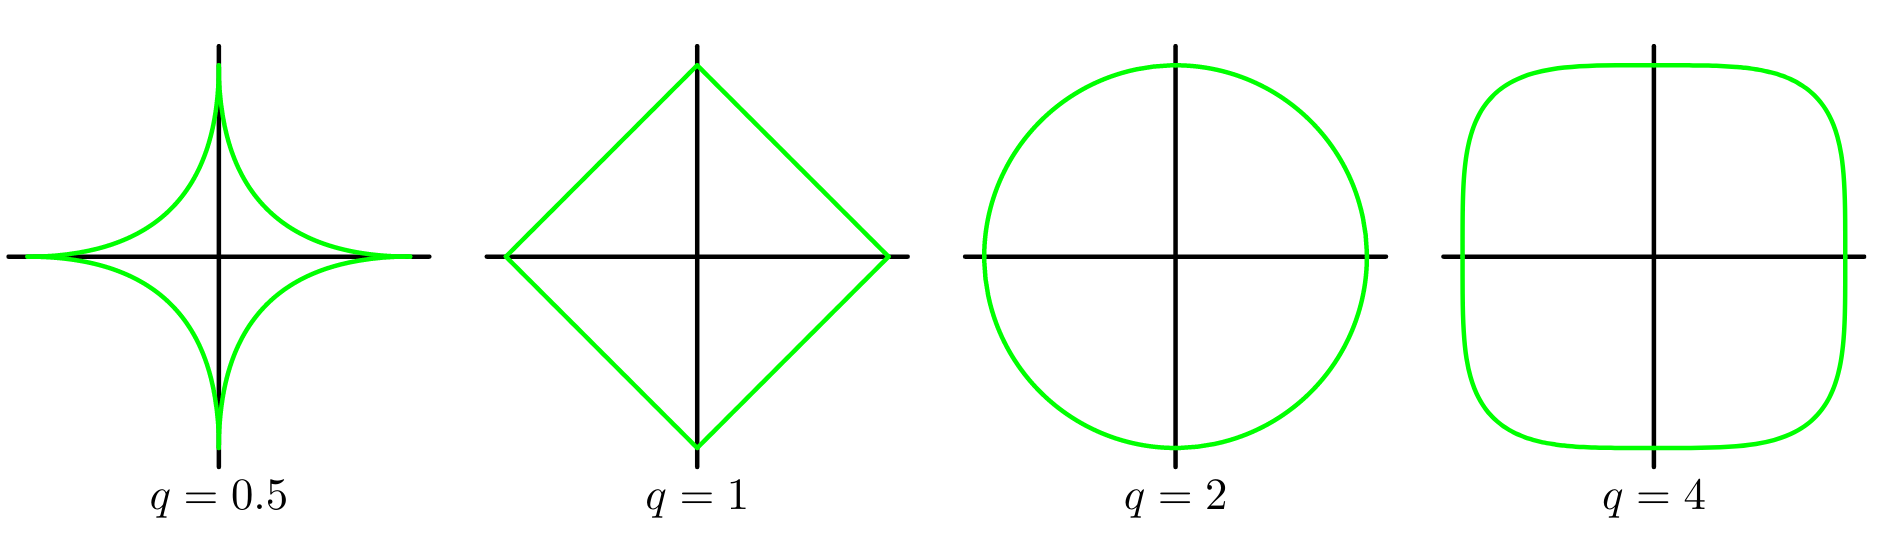
\includegraphics[width=0.7\columnwidth]{sl/1.png}
\end{figure}


解LASSO先考虑一个特殊的情况:$\Phi^T\Phi = I$,此时最小二乘的解是$w_\mathrm{LS} = \Phi^Ty$
$$
\begin{aligned}
    &\min_w \frac{1}{2}\sum^N_{i=1}(y_i - \bm w^T\bm\phi(\bm x_i))^2 + \lambda\|\bm w\|_1 \\
    &=\! \min_w \frac{1}{2}\sum^N_{i=1}(y_i\! - (w_\mathrm{LS}\! - w_\mathrm{LS}\! +\! \bm w)^T\bm\phi(\bm x_i))^2\! +\! \lambda\|\bm w\|_1 \\
    &\to \min_w \frac{1}{2}(\bm w - w_\mathrm{LS})^2 + \lambda\|\bm w\|_1 \\
\end{aligned}
$$
所以解为${w_\mathrm{lasso}}_i = \mathrm{sign}({w_\mathrm{LS}}_i) \max (|{w_\mathrm{LS}}_i| - \lambda, 0)$

Best subset: Hard thresholding,
Ridge: Uniformly shrink,
LASSO: Soft thresholding.

% \paragraph{贝叶斯方法} 
% 先定义先验$p(w) = \mathrm{N}(w|m_0, S_0)$,


\section{线性分类}

\paragraph{分类算法的分类}二分类、多分类、多标签分类(多个二分类的聚合)

\paragraph{分类和回归} 都想研究两个变量间的关系,离散情况就是分类了。分类需要量化,保证离散的输出。如果用普通的回归做分类,需要使用sign函数量化,但是这很难解。

\paragraph{逻辑回归} 使用sigmoid函数$\frac{1}{1+e^{-x}}$替代sign(),易解了很多。需要重新映射$y_i = \frac{t_i + 1}{2}$,并且使用交叉熵函数而不是平方误差之和:$\min_{\bm w, b} \sum_i - y_i\log\hat{y_i} - (1-y_i)\log(1-y_i)。$

\paragraph{交叉熵} 逻辑回归不是回归到特定的类别号,而是回归出一个属于某类的概率。这个概率的似然函数$P(t_i|x_i,\bm w,b) = \hat{y_i},\text{ if }t_i = +1\text{ else if }t_i = -1, 1 - \hat{y_i}$。
可以改写成$\hat{y_i}^{y_i}\cdot(1-\hat{y_i})^{(1-y_i)}$,然后取对数似然即可获得交叉熵。

其他解释:有两个概率分布,一个是ground-truth $P(t)$,一个是predicted $Q(t)$,那么交叉熵$C(P,Q) = \sum_tP(t)(-\log Q(t))$,熵$H(P)=\sum_tP(t)(-\log P(t))$,K-L散度(相对熵,两个分布的差异度,但是不对称$D_{KL}(P||Q) \neq D_{KL}(Q||P)$,$\ge 0$)$D_{KL}(P||Q) = C(P,Q) - H(P) = \sum_tP(t)\log{\frac{P(t)}{Q(t)}}$

\paragraph{解释逻辑回归}逻辑回归的预测值满足:
$$
\begin{array}{ll}
\hat{y_i} &= p(t_i = +1 |\bm x_i) \\
&= \frac{p(x_i|t_i=+1)p(t_i=+1)}{p(x_i|t_i=+1)p(t_i=+1) + p(x_i,t_i=-1)} \\
& = \frac{1}{1+e^{-(\bm w^T\bm x_i + b)}}
\end{array}
$$
$$\bm w^T\bm x_i + b = \ln \frac{p(\bm x_i| t_i = +1)p(t_i = +1)}{p(\bm x_i| t_i = -1)p(t_i = -1)} = \text{log odds},$$
几率,就是发生和不发生的比值,逻辑回归使用了对数几率(log odds)。
假设$p(x|t_i=k)$是高斯分布,则有:
$$\text{log odds} = \Sigma^{-1}(\mu_{+1}-\mu_{-1})\bm x_i + b$$

\paragraph{指数族} 指概率分布可以写成这样的分布:
$$p(\bm x|\bm \vartheta) = h(\bm x)g(\bm\vartheta)\exp(\bm\vartheta^T\bm\phi(\bm x)),$$
其中,$h(\bm x)$是,$\bm\vartheta$是自然参数,$\bm\phi(\bm x)$是充分统计量(为了估计分布所需要的统计量)。

\begin{table}[H]
\centering
\begin{tabular}{lll}
    \toprule
    分布 & 自然参数 & 充分统计 \\
    \midrule
    伯努利 & $\ln(p/(1-p))$ & $x$ \\
    泊松 & $\ln\lambda$ & $x$ \\
    指数 & $-\lambda$ & $x$ \\
    拉普拉斯 & $-1/b$ & $|x-\mu|$ \\
    \bottomrule
\end{tabular}
\end{table}
累积函数$\bm A(\bm\vartheta) = - \ln \bm g(\bm \vartheta)$,有以下性质:
$$
\begin{array}{l}
    \frac{\partial\bm A}{\partial \vartheta_i} = \mathbb{E}[\bm\phi_i(\bm x)] \\
    \frac{\partial^2\bm A}{\partial \vartheta_i\partial \vartheta_j} = \mathbb{E}[\bm\phi_i(\bm x)\bm\phi_j(\bm x)] - \mathbb{E}[\bm\phi_i(\bm x)]\mathbb{E}[\bm\phi_j(\bm x)]
\end{array}
$$
也就是说偏导数是均值、二阶偏导数是协方差,这样的分布具有最大熵的特性。

\paragraph{最大熵}
具有最大微分熵性质的分布是高斯分布,具有最大熵性质的离散分布是均匀分布。

\paragraph{求解逻辑回归} 其最小二乘的梯度为:
$$\nabla E(\bm w) = \sum_i (\hat{y_i} - y_i)\bm \phi(\bm x_i),$$
所以,没有解析解(封闭解)。

\paragraph{优化问题的数值解法} 
\begin{enumerate}
    \item 二阶:Newton-Raphson
    \item 一阶:Gradient Descent, Frank-Wolfe
\end{enumerate}

牛顿法,由泰勒的二阶展开,并令一阶导数为零可得:
$$x^{\prime} = x - H^{-1}\nabla f(x),$$
其中,$H$是海森矩阵。

梯度下降,由泰勒一阶展开,令一阶导数为零可得:
$$x^{\prime} = x -\eta\nabla{}f(x)$$

Frank-Wolfe,求解约束优化问题,也是一阶泰勒展开,考虑$s_t = \min xf^\prime(x_t)$,找到$s_t$之后,每步找到个系数$\gamma \in (0,1)$:
$$x_{t+1} = \gamma s_t - (1-\gamma)x_t$$

\paragraph{费雪线性判别分析(LDA)} 最大化类之间的间距、最小化类内的方差,这在几何上也行得通。经分析其是高斯-逻辑回归的近似。

\paragraph{感知机} 可以用梯度下降解
$$\min_{w,b} \sum_{i=1}^N (t_i - \mathrm{sign}(\bm w^T\bm x_i + b)).$$

\paragraph{多分类--用二分类模拟}数据集划分时总是有未分类的例子
\begin{enumerate}
\item one-versus-the-rest
\item one-versus-one
\end{enumerate}

\paragraph{多分类--softmax回归} 
和前面解释差不多,只不过:
$$\hat{y_i}_k = p(t_i = k|x_i) = \frac{p(x_i|t_i = k)p(t_i = k)}{\sum_m p(x_i|t_i = m)p(t_i = m)},$$
定义$\ln p(x_i|t_i = k)(t_i = k) = {w_k}^Tx_i + b_k$,这就是softmax回归

\paragraph{多标签分类} 就是多个二分类器连接在一块

\section{SVM}
\paragraph{硬边际SVM} 思想是最大化类之间的边际,这样对噪声不敏感且有最好的泛化能力。找到离分类边界最近的点到边界的距离:
$$\gamma = \min_i \frac{y_i(\bm w^T\bm x_i + b)}{\|\bm w\|}$$,我们使最近的点的$y_i(\bm w^T\bm x_i + b) = 1$(通过缩放系数,这些点叫做支持向量),那么显然需要最大化$1/\|\bm w\|$,也就是:
$$\min_{w,b} \frac{1}{2}\|\bm w\|^2, \text{s.t.} 1 - y_i(\bm w^T\bm x_i + b) \le 0,$$
其拉格朗日函数为:
$$L(\bm w, \bm x, \bm \alpha) = \frac{1}{2}\|\bm w\|^2 - \sum_i \bm \alpha_i(y_i(\bm w^T\bm x_i + b) - 1),$$套KKT,结果如下:
$$\begin{array}{l}
\bm w = \sum_i \alpha_iy_i\bm x_i, \\
\sum_i \alpha_iy_i = 0, \\
\alpha_i \ge 0, \\
y_i(\bm w^T\bm x_i + b) \ge 1, \\
\alpha_i(y_i(\bm w^T\bm x_i + b) - 1) = 0,
\end{array}$$
也就是,要么$\alpha_i = 0$,要么$\bm w^T\bm x_i + b = \pm 1$(此时$\bm x_i$是支持向量)。
\paragraph{对偶问题}
$$\max_\alpha\min_{\bm w, b} \frac{1}{2}\|\bm w\|^2 - \sum_i \bm \alpha_i(y_i(\bm w^T\bm x_i + b) - 1),$$
套KKT,结果如下:
$$
\begin{array}{l}
\max_\alpha \sum_i \alpha_i - \frac{1}{2}\sum_i\sum_j \alpha_i\alpha_jy_iy_j\bm{x}_i^T\bm{x}_j, \\
\text{s.t.} \forall \alpha_i \ge 0, \sum_i \alpha_iy_i = 0 \\
\bm w = \sum_i \alpha_iy_i\bm x_i \\
b = y_i - \bm w^T \bm x_i
\end{array}
$$

\paragraph{软边际SVM} 如果非线性可分,我们应该使用软边际SVM。此时我们会对错误分类的点、还有过于靠近分类面的点进行容忍。
$$\min_{w,b} \frac{1}{2}\|\bm w\|^2, \text{s.t. } \mathrm{Ind}(y_i(\bm w^T\bm x_i + b) - 1) \le c_0,$$
其中,Ind函数是指示函数,仅在小于0时得1。也就是说$y_i(\bm w^T\bm x_i + b) \le 1$时有效。那么可以写成另外一种形式:
$$
\min_{w,b} \frac{1}{2}\|\bm w\|^2 + C\sum_i \xi_i, \text{s.t.}\xi_i \ge 0, y_i(\bm w^T\bm x_i + b) \ge 1 - \xi_i,
$$
其中,$\xi = \max(0, 1-y_i(\bm w^T\bm x_i + b))$,叫做松弛变量。其拉格朗日函数如下:
$$
L(\bm w, \bm x, \xi, \bm \alpha, \bm \beta) = \frac{1}{2}\|\bm w\|^2 - \sum_i \bm \alpha_i(y_i(\bm w^T\bm x_i + b) - 1),
$$
套KKT,结果如下:
$$
\begin{array}{l}
\bm w = \sum_i \alpha_iy_i\bm x_i, \\
\sum_i \alpha_iy_i = 0, \\
\alpha_i + \beta_i = C \Rightarrow 0 \le \alpha_i \le C, \\
\alpha_i \ge 0, \beta_i \ge 0, \xi_i \ge 0, \beta_i\xi_i = 0\\
y_i(\bm w^T\bm x_i + b) \ge 1 - \xi_i, \\
\alpha_i(y_i(\bm w^T\bm x_i + b) - 1 + \xi_i) = 0, 
\end{array}
$$
对偶问题如下:
$$
\begin{array}{l}
\max_\alpha \sum_i\alpha_i - \frac{1}{2} \sum_i\sum_j\alpha_i\alpha_jy_iy_j\bm{x}_i^T\bm{x}_j, \\
\text{s.t. }0 \le \alpha_i \le C, \sum_i \alpha_i y_i = 0,
\end{array}
$$
也就是说,$C = +\infty$时,就是硬边际SVM,样本分为三类,后两类是支持向量:
$$
\left\{
\begin{array}{ll}
\alpha_i = 0, & \xi_i = 0, y_i(\bm w^T\bm x_i + b) > 1 \\
0 < \alpha_i < C, & \xi_i = 0, y_i(\bm w^T\bm x_i + b) = 1 \\
\alpha_i = C, & \xi_i > 0, y_i(\bm w^T\bm x_i + b) < 1
\end{array}
\right.
$$
\paragraph{核技巧}
把上文中所有$\bm x_i$换成$\bm\phi(\bm x_i)$,即可获得基函数版本的SVM。将上文中的$\bm{x}_i^T\bm{x}_j$换成$k(\bm x_i, \bm x_j)$,可以得到核函数版本的SVM。其实核函数满足:
$$k(\bm x_i, \bm x_j) = \bm\phi(\bm x_i)^T\bm\phi(\bm x_j),$$
常见的核函数有线性$\bm x_i^T\bm x_j$、RBF$\exp(-\|\bm x_i - \bm x_j\|^2/2\sigma^2)$、多项式$(1+\bm x_i^T\bm x_j)^p$、sigmoid核$\tanh(\alpha\bm x_i^T\bm x_j+\beta)$。

使用核函数与使用基函数并无什么不同,相反核函数还较基函数容易表示一些。满足Mercer's condition就是核函数,也就是说是必须是正定的:
$$\int_{\bm x}\int_{\bm y}f(\bm x)K(\bm x, \bm y)f(\bm y)\mathrm{d}\bm x\mathrm{d}\bm y > 0, \forall f$$

\paragraph{SMO算法}
序列最小优化算法,每次选择两个拉格朗日乘子作为变量,其他的乘子不变。变量乘子都在“盒限制”中选取新值。是坐标下降,比梯度下降简单。

\section{监督学习}
前面我们学习了回归、分类、密度估计,这些都是完全的监督学习。
监督学习的基本方法:收集数据(清洗)$\rightarrow$决定模型形式(超参)$\rightarrow$决定策略/优化目标$\rightarrow$模型学习(获取参数)$\rightarrow$评价模型

\paragraph{判别模型和概率模型}
判别模型:$\hat{y} = f(x)$(分类、回归),概率模型$q(y|x)$(分类、回归、密度估计)。如果目标变量是离散的,就是分类问题;是连续的就是回归问题。

\paragraph{判别模型和生成模型}
判别模型:$\hat{y} = f(x)$或者$q(y|x)$,生成模型$\hat{x} = f(y)$或者$q(x|y)$。在监督学习中,生成模型不是必要的。如果两个模型都学习了,我们实际上完成了对$p(x,y)$的估计。密度估计在监督学习中是万能的,但是很难解决。判别模型方法只需要处理判别模型,并且可以很容易运用基/核函数,在小数据集上表现更好。生成模型方法需要处理判别模型和生成模型,可以使用隐变量,在处理大量数据时更加容易拟合。

\paragraph{损失函数} $\mathcal{L}(x_i,y_i,f)$,$f$是泛函,下面是一些例子:
\begin{itemize}
    \item 平方损失:$(y_i - f(x_i))^2$
    \item 绝对损失:$|y_i - f(x_i|^2$
    \item 0-1损失:$\text{if $y_i = f(x_i)$ then 0 else 1}$
    \item log损失,通常见于概率函数(逻辑回归):$-\log q(y_i|x_i)$
    \item 铰链损失,感知机:$\left\{\begin{aligned}
        0, \ \text{if}\ y_i(w^Tx_i +b) \ge 0, \\
        -y_i(w^Tx_i +b), \text{otherwise}
    \end{aligned}\right.$
    \item 铰链损失,SVM:$\left\{\begin{aligned}
        0, \ \text{if}\ y_i(w^Tx_i +b) \ge 1, \\
        1-y_i(w^Tx_i +b), \text{otherwise}
    \end{aligned}\right.$
\end{itemize}

\paragraph{风险函数}
设定输入空间$x\in \mathcal{X}$,输出空间$y\in \mathcal{Y}$,假设空间$f: \mathcal{X} \to \mathcal{Y}, f(x) \in \mathcal{H}$,参数化$f(x) \to f(x|\alpha)$,参数空间$\alpha \in \Lambda$。那么风险函数就是损失函数的函数$R: \Lambda \to \mathbb{R}$:
$$R(\alpha) = \int_{x\in \mathcal{X}, y\in \mathcal{Y}} L(x, y, \alpha)p(x,y) \mathrm{d}x\mathrm{d}y$$
风险最小化就是我们想要的,但是很难进行估计。

\paragraph{经验风险} 基于训练数据,我们用经验风险估计风险:
$$R_\text{emp}(\alpha) = \frac{1}{N} \sum^N_{i=1}L(x_i, y_i, \alpha),$$
其实最小二乘法、最大似然估计就是经验风险最小化(ERM)。有很多关于ERM的问题:
ERM可能会导致不适定问题,因此我们使用正则化。ERM 不能包含先验信息,因此我们使用贝叶斯。ERM不考虑数据集方差,因此我们使用偏差-方差权衡。ERM没有考虑模型存储的成本,所以我们使用
最小描述长度 (MDL)。ERM能保证风险最小化吗? 

\paragraph{过拟合} 原因如下:
\begin{itemize}
    \item 训练数据不足
    \item 数据有噪声
    \item 模型复杂度太高
\end{itemize}

\begin{figure}[H]
    \centering
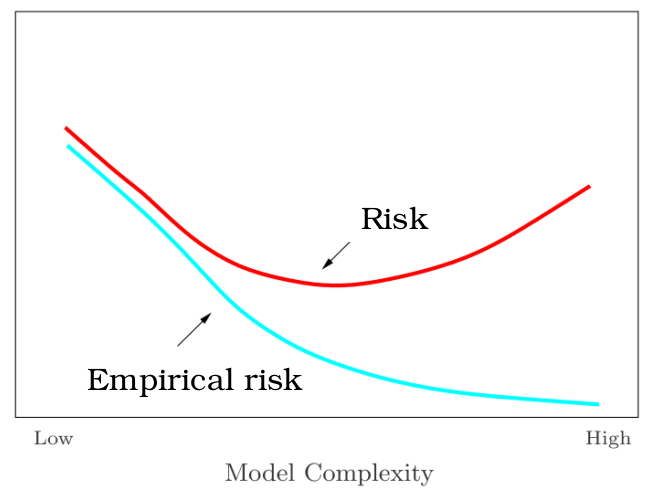
\includegraphics[width=0.7\columnwidth]{sl/2.png}
\end{figure}

\paragraph{风险和经验风险}
风险最小化$\alpha^*=\arg\min_{\alpha \in \Lambda} R(\alpha)$,依靠损失函数、概率测量、参数空间。经验风险最小化$\alpha_N=\arg\min_{\alpha \in \Lambda} R_\text{emp}(\alpha)$,依靠损失函数、训练数据、参数空间。

\paragraph{一致学习} 因为大数定理,所以风险和经验风险能够足够接近。前面$R_\text{emp}(\alpha_N) = 0$的最大样本数$N$点就是VC维的大小,代表100\%的拟合,也就是最大能打散的样本数,
%VC维也叫做函数集的熵。
\begin{figure}[H]
    \centering
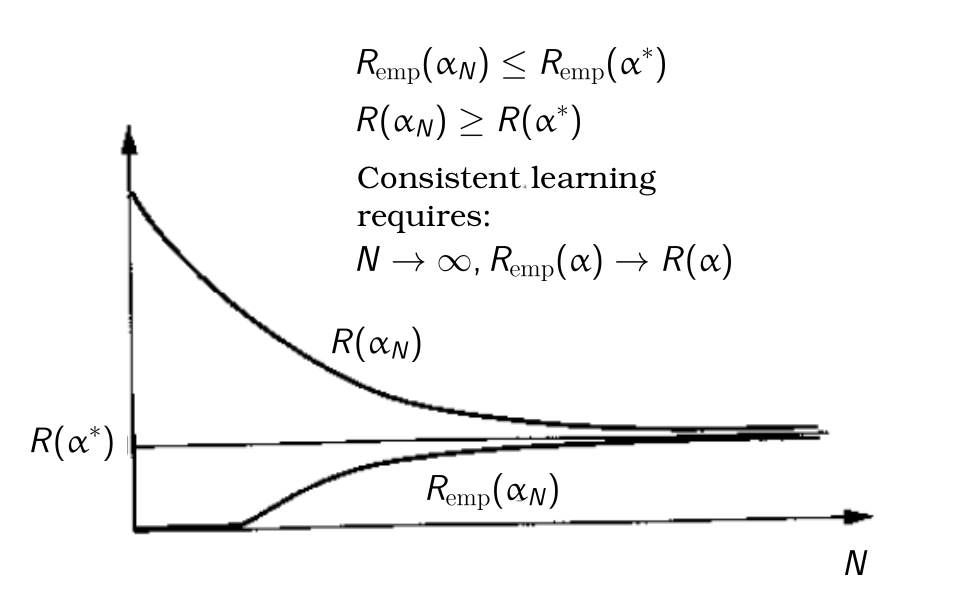
\includegraphics[width=0.7\columnwidth]{sl/3.png}
\end{figure}

举个特殊例子,如果参数空间只有一个参数$\alpha_0$,那么根据Hoeffding不等式(且采用0-1 loss)有:
$$P(R(\alpha_0) - R_\text{emp}(\alpha_0)) \le \exp(-2N\epsilon^2),$$
或者说,至少以$1-\eta$的概率有:
$$R(\alpha_0) \le R_\text{emp}(\alpha_0) + \sqrt{\frac{-\log \eta}{2N}},$$
那么更加一般的情况下,假设有M个有限参数,我们至少以$1-\eta$的概率有:
$$
\sup_{\alpha \in \Lambda}(R(\alpha) - R_\text{emp}(\alpha)) \le \sqrt{\frac{1}{2N}(\log M - \log \eta)},
$$
但是有些实用的学习模型有无限数量的参数!

\paragraph{函数集的熵}
考虑二分类$f(x|\alpha) \in \{-1,+1\}$,当我们给定一个数据集和一个参数空间时有多少种可能的结果?定义:
$\mathcal{N}^{\Lambda}(x_1, x_2, \ldots, x_N) = \mathrm{Count}\{(f(x_1|\alpha), \ldots, f(x_N|\alpha)) | \alpha \in \Lambda\},$
注意,我们同样可以根据损失函数(0-1 loss)来定义这个数字,并且这个数字是相等的。

我们定义熵为$H^\Lambda(N) = \mathbb{E}_{x\in \mathcal{X}} \log(\mathcal{N}^\Lambda)$,退火熵为$H_\mathrm{ann}^\Lambda(N) = \log(\mathbb{E}_{x\in \mathcal{X}} \mathcal{N}^\Lambda) > H^\Lambda(N)$,生长函数为$G^\Lambda(N) = \log(\sup_{x\in \mathcal{X}} \mathcal{N}^\Lambda)$。

理论1:一致学习\\
当且仅当$\lim_{N\to \infty} \frac{N^\Lambda}{N} = 0,$而且$\lim_{N\to \infty} P(|\sup_{\alpha \in \Lambda}(R(\alpha) - R_\text{emp}(\alpha))| > \epsilon) = 0, \forall \epsilon > 0$。

理论2:快速收敛\\
如果$\lim_{N\to \infty} \frac{H_\mathrm{ann}^\Lambda(N)}{N} = 0,$那么$P(R(\alpha_N) - R(\alpha^*) > \epsilon) < \exp(-c\epsilon^2N), \forall \epsilon > 0, \forall N > N_0$

理论3:
当且仅当$\lim_{N\to \infty} \frac{G^\Lambda(N)}{N} = 0,$那么学习是一致的而且收敛是快速的,不管$p(x)$是什么。

\paragraph{VC维度}
我们可以进一步证明任何生长函数都要么满足$G^\Lambda(N) = N\log 2$,或者$G^\Lambda(N) \le h(\log (N/h) + 1)$,其中$h$是个整数且有$G^\Lambda(h) = h \log 2, G^\Lambda(h+1) < (h+1)\log 2$,$h$就是VC维度。VC维度的就是函数集可以打散的最多样本的数量$h$。

在$D$维的线性分类器中,其VC维为$D+1$。此时VC维与其参数的数量一样。

拥有可以调节频率的$\sin()$的模型,其VC维是无穷的!

SVM需要考虑一个受限的线性分类器:$$y=\left\{\begin{aligned} 
+1, \text{if}\ w^Tx+b\ge \Delta, \\
-1, \text{if}\ w^Tx+b\le \Delta,
\end{aligned}\right.$$的VC维是$h \le \min(D, [\frac{R^2}{\Delta^2}]) + 1$,$R$是能覆盖所有数据点的超球体的半径,小于线性分类器,其拟合能力比较弱。

直观地说,VC维度表征了一个函数集的强大程度。无限VC维度意味着,对于特定数据集,函数集总是可以实现等于0的经验风险,即 ERM不提供信息。严格地,VC维定义了风险的边界。
$$
\epsilon = 4\times \frac{h(\log(2N/h)+1) - \log(\eta/4)}{N},
$$
$$
\sup_{\alpha \in \Lambda}(R(\alpha) - R_\text{emp}(\alpha)) \le \sqrt{\frac{\epsilon}{4}},
$$
对于有限的参数空间,我们有$\epsilon = 2 \times \frac{\log M - \log \eta}{N}$

VC维度描述了无限函数集的“有效体积”。
但是许多重要分类器(决策树、神经网络)的VC维度尚不清楚,
VC维度分析不适用于非参数学习(例如 k-NN)。

\paragraph{结构风险最小化}
SRM试图最小化ERM和置信区间的总和。SRM是正则化的一个具体例子
$$\min_\alpha R_\text{emp}(\alpha) + \lambda C(\alpha)$$
其中,正则化项控制了模型的复杂度。正则化首先被提出来处理病态问题。有几种不同的方式来解释/执行正则化:贝叶斯、偏差-方差均衡、最小描述长度(MDL)。

\paragraph{贝叶斯作为正则化手段}
考虑概率建模$q(y|x)$
,损失函数是对数损失$-log q(y_i|x_i)$。
最小化经验风险就是极大似然,最大化后验$p(\alpha | \{x_i, y_i\}_{i = 1,\ldots, N})$,
需要先验$p(\alpha)$。
因此,正则化项等价于$-\log p(\alpha)$

贝叶斯与SRM对比\\
• 贝叶斯需要先验信息\\
• SRM不要求真实模型位于假设空间内 

\paragraph{偏差-方差均衡作为正则化手段} ERM没有考虑数据集的方差,这是类似于正则项的地方。但是偏差-方差均衡难以实现。

\paragraph{最小描述长度作为正则化手段} 最小描述长度(MDL)原则:最佳模型是在给定数据集上能够达到最小描述长度的模型。MDL考虑了模型存储的成本,相当于正则化项。MDL需要适当的编码规则;但是理想的编码与概率有关。

\paragraph{精度、召回率、AUC}
对于二元分类,我们通常希望区分不同类型的错误。
$$\text{Precision} = \frac{\text{TP}}{\text{TP} + \text{FP}}$$
$$\text{Recall} = \frac{\text{TP}}{\text{TP} + \text{FN}}$$
$$\text{F1-value} = \frac{2\times\text{Precision}\times\text{Recall}}{\text{Precision} + \text{Recall}}$$
最理想情况下,FN=FP=0。

还有一个AUC,它是ROC (receiver operating characteristic) curve的曲线下面积。ROC曲线的X轴是$\frac{\text{FP}}{\text{FP} + \text{TN}}$,Y轴是$\frac{\text{TP}}{\text{TP} + \text{FN}}$(Recall)。随机的二分类器AUC为0.5,理想的为1。

\section{非参数学习}
许多统计学习方法假设了个模型,其学习过程就是解出或者估计出模型的参数。非参数学习没有明面上的模型,有时被称为基于实例/记忆的学习。
\paragraph{Parzen Window/核密度估计}
求解(概率)密度估计问题,给出一组样本$x_1,\ldots,x_N$,求$p(x)$。PW用核函数(需要满足非负、积分为1,比如说,高斯核)求和来估计:
$$\hat{p}(x) = \frac{1}{N}\sum^N_{i=1}K(x|x_i),$$
其实PW和直方图很像,一个是经验概率密度函数,一个是用核函数的相加估计真正的PDF。那么我们也需要一个超参数$h$用于控制窗口大小:
$$
\begin{array}{l}
K_h(x) = \frac{1}{h}K(\frac{x}{h}) \\
\hat{p}_h(x) = \frac{1}{N}\sum^N_{i=1}K_h(x|x_i),
\end{array}
$$
窗越小,越容易过拟合。

\paragraph{$k$-NN}看空间关系最近的$k$个样本,(简单/加权)投票决定样本归属哪一类。设$\mathcal{N}(x_i)$是$x_i$的邻居。
$$
\begin{array}{ll}
\text{分类} & \hat{y} = \mathrm{sign}(\sum_{x_i \in \mathcal{N}(x_i)} y_i) \\
\text{回归} & \hat{y} = \frac{1}{|\mathcal{N}(x_i)|} \sum_{x_i \in \mathcal{N}(x_i)} y_i \\
\end{array}
$$
1-NN对噪声太过敏感。用偏差-方差分解考察k-NN回归$\mathbb{E}[(\hat{y} - y)^2]$,发现同样有偏差-方差-噪声三项。$k\uparrow,\text{var} \downarrow,\text{bias} \uparrow$

\paragraph{稀疏编码} 目的是要求解:
$$x = \sum^N_{i=1} \alpha_ix_i,\text{ s.t. } \|\alpha\|_0 \le k,$$
可以放宽以处理数据中的噪声或损坏。

\section{无/半监督学习}
有监督学习意图找出数据之中的关系以解决预测问题。无监督学习意图发现数据中的模式,以对数据进行描述:比如关联分析(啤酒尿布,什么属性是互相关联的)、聚类(分类的弱化版)、异常检测(数据是否是正常的)、降维(避免维度诅咒)等等

\paragraph{维度诅咒}
\begin{enumerate}
    \item 在高维空间,距离无法区分 
    \item 最近的邻居都在很远的地方
\end{enumerate}
为什么?因为高维空间非常大,样本很稀疏。

\paragraph{K-means} 是Prototype-based clustering的代表。每个聚类都有个原型,样本距离原型的距离决定了样本的类别。
\begin{algorithm}[H]
\caption{K-means算法}
\label{alg:K-means}
\begin{algorithmic}[1]
\Require dataset $\{x_1, \ldots, x_N\}$, number of clusters $k$
\Ensure clusters $q(x_i)\in\{1, \ldots, k\}$
\State Initialize centroids $\{c_1, \ldots, c_2\}$
\Repeat
\For{$i = 1, \ldots, N$}
\State $q(x_i) \leftarrow \arg \min_j |x_i - c_i|$
\EndFor
\For{$i = 1, \ldots, k$}
\State $c_j \leftarrow \mathrm{mean}(x_i|q(x_i) = j)$
\EndFor
\Until{centroids do not change}
\end{algorithmic}
\end{algorithm}
通常来说这个算法会收敛。

中心点(也就是前面的prototype)也被称为码字,组成码本。k-means其实是解决
$$\min_{q,\{c_j\}} |x_i - c_{q(x_i)}|^2$$
k-means算法启发式地交替更新$q$和$\{c_j\}$。这是贪心的,不能保证得到全局最优解。经常受到离群点、不同大小的簇、不同密度的簇、不规则形状的影响。一个办法是过分割(增大$k$),然后再后处理。

\paragraph{高斯混合模型}
高斯混合模型是一种基于分布的聚类方法。每一个簇代表一个单模态的分布。计算后验概率以决定样本属于哪一个簇。在高斯混合模型中,每个分布是高斯分布。\begin{enumerate}
    \item 一维情况:$p(x) = \sum_{j=1}^k w_j\mathcal{N}(x|\mu_j, \sigma_j^2),\text{ where} \sum_j w_j = 1,$
    \item 多维情况:$p(x) = \sum_{j=1}^k w_j\mathcal{N}(x|\mu_j, \Sigma_j),\text{ where} \sum_j w_j = 1,$
\end{enumerate}
如果我们知道了GMM的参数,那么我们可以这样计算后验概率(也叫响应度):
$$p(q(x_i) = j) = \gamma_{ij} = \frac{w_j\mathcal{N}(x|\mu_j, \sigma_j^2)}{\sum_{j=1}^kw_j\mathcal{N}(x|\mu_j, \sigma_j^2)},$$
然后有$q(x_i) = \arg\max_j \gamma_{ij},$
所以说,我们怎么样估计GMM的参数$\theta = \{w_j, \mu_j, \Sigma_j | j = 1, \ldots k\}$呢?

问题就是要最大化$\prod_{i=1}^N \sum_{j=1}^k w_j \mathcal{N}(x_i|\mu_j, \Sigma_j)$,我们可以借鉴K-means的算法。首先初始化参数,然后计算相应的相应度,第三步更新参数。上面两个步骤交替进行,直到模型收敛。

记$\gamma_{ij} = p(q(x_i) = j)$:$$
\begin{aligned}
    w_j = \frac{\sum_i \gamma_{ij}}{N} \\
    \mu_j = \frac{\sum_i \gamma_{ij}x_i}{\sum_i \gamma_{ij}} \\
    \Sigma_j = \frac{\sum_i \gamma_{ij}(x_i - \mu_j)^T(x_i - \mu_j)}{\sum_i \gamma_{ij}} \\
\end{aligned}
$$

\paragraph{EM算法}
引入隐变量$z_i \in \{1, \ldots, k\}$,代表$x_i$对应的正确的簇,那么要最大化$\prod_i p(x_i, z_i|\theta) = \prod_i \prod_j (w_j\mathcal{N}(x_i|\mu_j, \Sigma_j))^{\mathcal{I}(z_i =j)}$,或者$\sum_i \sum_j \mathcal{I}(z_i =j)\log(w_j\mathcal{N}(x_i|\mu_j, \Sigma_j))$

EM算法分为交替的两步:E-step: Given $\theta^t$, calculate the expectation of object function with
eliminating latent variables. Note that $\gamma_{ij}$ is the expectation of $\mathcal{I}(z_i = j)$, so we have $\sum_i\sum_j \gamma_{ij} \log(w_j\mathcal{N}(x_i|\mu_j, \Sigma_j))$

M-step: Maximize the expectation of objective function to find a new estimate of parameters $\theta^t$. Then we can derive the equations of GMM

\begin{algorithm}[H]
\caption{EM算法}
\label{alg:EM}
\begin{algorithmic}[1]
\Require $\hat{\theta} = \max_\theta p(X,Z|\theta)$, where $Z$ is unobserved
\State $t \leftarrow 0$, initialize $\theta^0$
\Repeat
\State Given $\theta^t$, calculate the expectation of $\log p(X, Z|\theta)$ with eliminating $Z$, i.e. $Q(\theta, \theta^t) = \mathbb{E}_{Z\sim p(Z|X, \theta^t)}\log p(X, Z|\theta)$
\State $\theta^{t+1} \leftarrow \arg \max_{\theta} Q(\theta, \theta^t)$
\Until{convergence}
\State $\hat{\theta} = \theta^{t+1}$
\end{algorithmic}
\end{algorithm}
EM is a greedy algorithm, it will definitely converge but cannot ensure global optimum.

Set different initial values to escape from a local optimum. We may not maximize the expectation (i.e. the Q function); instead, increasing the Q function (e.g. by gradient ascent) is okay; this can be helpful if the Q function is not easy to maximize.

\paragraph{不同的聚类方法}
基于密度的聚类:Mean-shift: 局部密度的均值来替代;DBSCAN:对于每个点,如果邻点的数目小于一个阈值,那么这个点就是噪声。否则,属于一个簇/基于连通性的聚类/Agglomerative clustering/Divisive clustering

\paragraph{PCA}
给出一个$x\in \mathbb{R}^D$,我们想要找到一个矩阵$P \in \mathbb{R}^{K \times D}$,其中$K < D$,然后我们可以用这个矩阵$P$降维$x$:$y = Px, y \in \mathbb{R}^K$。

第一步是$\bar{x} = \frac{\sum_i x_i}{N}$,令$X = \begin{pmatrix}
    (x_1 - \bar{x})^T \\
    \cdots \\
    (x_N - \bar{x})^T
\end{pmatrix}$,
第二步是$C = X^TX = U\Lambda U^H$,这是个协方差阵,可以找出其特征值和特征向量,第三步是选择最大的K项特征值,并且选择对应的特征向量组成$P$,$y_i = P(x_i - \bar{x})$

\paragraph{核PCA}
对于非线性,使用核函数实现。$\Phi = \begin{pmatrix}
    \phi_i^T \\
    \cdots \\
    \phi_N^T
\end{pmatrix}$,其中$\phi_i = \phi(x_i)$。我们关心的是$K = \Phi\Phi^T$。

\paragraph{流形学习}
流形是一种拓扑空间,它在每一点附近都与欧几里得空间相似。
一维流形包括线和圆,但不包括"8"。
二维流形也被称为曲面,如球体。
流形的内在维度可以低于它的驻留空间。
流形学习是为了从高维数据中识别这种低维结构。
对于流形学习,用测地线距离代替高维欧几里得距离。

% TODO

\paragraph{PageRank} 基于Random Walk,用来定义网页的相对重要度的。
\begin{algorithm}[H]
\caption{PageRank算法}
\label{alg:PageRank}
\begin{algorithmic}[1]
\Require A graph of webpages and hyperlinks
\Ensure Relative importance values of all webpages
\State $t \leftarrow 0$, initialize $r_i^0$ uniformly
\Repeat
\State $\forall j, r_j{t+1} \leftarrow 0$
\State $\forall i,j, \mathrm{if}\ w_{ij} \neq 0, r_j^{t+1} = r_j^{t+1} + \frac{w_{ij}}{\sum_k w_{ik}}r_i^t$
\State $\forall j, r_j^{t+1} \leftarrow \beta r_j^{t+1} + \frac{1-\beta}{N}$
\Until{convergence}
\end{algorithmic}
\end{algorithm}

\section{组合学习}
建立多个个体/基础学习器,然后将它们组合起来。当这些基础学习器好而不同的时候,组合学习很有效果。但是实际中,基础模型们很难做到独立。我们希望每个基础模型尽可能不同,但是多元化和性能是冲突的。有两种形式的组合学习:
\begin{enumerate}
    \item Boosting: 每个基础模型都顺序地训练,整体模型更加关注模型之前处理得不太好的样本。
    \item Bagging: 每个模型都是独自、并行地训练,整体模型尝试使每个基础模型的训练数据多样化。
\end{enumerate}

\paragraph{Boosting}
$$f_m(x) = f_{m-1}(x) + \alpha_mG_m(x),$$
其中$G_m(x)$是基础模型,那么整体模型是
$$f(x) = \sum_m \alpha_m G_m(x)$$

\paragraph{Boosting回归树}
$$f(x) = \sum_m \alpha_m T(x, \theta_m),$$
其中,$T(x,\theta_m)=\left\{\begin{array}{ll}
    c_{m1}, & \text{if }x \le t_m, \\
    c_{m2}, & \text{if }x > t_m,
\end{array} \right.$是决策树桩。我们利用残差训练该模型,算法如下:
\begin{algorithm}[H]
\caption{Step-wise learning algorithm}
\label{alg:step-wise}
\begin{algorithmic}[1]
\Require $\{x_n, y_n\}$
\Ensure $\{\alpha_m, \theta_m\}$
\For{$m=1, \ldots, M$}
\State Calculate residue ${r_n}^{(m)} = y_n - f_{m-1}(x_n)$
\State Fit the residue with decision stump $T(x,\theta_m)$
\State Set $\alpha_m = 1$
\State Update the model $f_m(x) = f_{m-1}(x) + \alpha_mT(x, \theta_m)$
\EndFor
\end{algorithmic}
\end{algorithm}

\paragraph{\textit{Ada}ptive \textit{Boost}ing}
分类模型,目标是优化:
$$\sum_{n=1}^N \mathcal{L}(y_n, f(x_n)) = \sum_{n=1}^N \exp(-y_n \times f(x_n)),$$
最小化$\sum^N_{n=1} \mathcal{L}(y_n, f(x_n)) = \sum_{n=1}^N \exp(-y_n \times f(x_n)),$也就是:
$$
\sum_{n=1}^N \exp(-y_n \times [f_{m_1}(x_n) + \alpha_mG_m(x_n)]),
$$

\begin{algorithm}[H]
\caption{AdaBoost Algorithm}
\label{alg:AdaBoost}
\begin{algorithmic}[1]
\Require $\{x_n, y_n\}$
\Ensure $f(x) = \sum_m \alpha_mG_m(x)$
\For{$m=1, \ldots, M$}
\State Calculate weights of samples: $w_{mn} = \exp(-y_n \times f_{m-1}(x_n))$ and then
normalize $w_{mn} \leftarrow \frac{w_{mn}}{\sum_n w_{mn}}$\begin{itemize}
    \item $m=1$, then $w_{1n} = 1/N$
    \item $w_{(m+1)n} \propto w_{mn}\exp(-y_n\alpha_mG_m(x_n))$
\end{itemize}
\State $G_m(x)$ is to minimize $e_m = \sum_{n=1}^N w_{mn}\mathbb{I}(y_n \neq G_m(x_n))$
\State $\alpha_m = \frac{1}{2} \log \frac{1-e_m}{e_m}$
\EndFor
\end{algorithmic}
\end{algorithm}

如果一个样本被正确分类,其权重就会减少$exp(-alpha_m)$。
如果一个样本被错误地分类,它的权重会增加$exp(-alpha_m)$。
因此,下一个基础分类器将专注于错误分类的样本。

\paragraph{Bagging = bootstrap aggregating} 通过自举采样生成多个数据集。生成$M$个数据集,用每个数据集来训练一个模型。然后对它们进行平均:$f(x) = \frac{1}{M} \sum_m G_m(x)$,可以并行学习。

\section{决策树}
树模型由一组条件和一组基本模型组成,以树的形式组织起来。每个内部节点都是一个针对输入属性的条件——对输入空间的划分。每个叶子节点就是一个基本模型,回归时最简单为一个常数,分类时最简单为一个类别。

\paragraph{构建决策树} 是个NPH问题。所以穷尽搜索不可行,我们应该用启发式方法,如下:
\begin{algorithm}[H]
\caption{Hunt's algorithm}
\label{alg:hunt}
\begin{algorithmic}[1]
\Require A set of training data $\mathcal{D} = \{x_n, y_n\}$
\Ensure A classification tree or regression tree T
\Function{HuntAlgorithm}{$\mathcal{D}$}
\If{$\mathcal{D}$ need not or cannot be divided}
\State \Return a leaf node
\Else
\State Find an attribute of $x$, say $x_d$, and decide a condition $g(x_d)$
\State Divide $\mathcal{D}$ into $\mathcal{D}_1, \mathcal{D}_2, \ldots$, according to the output of $g(x_d)$
\State $T_1 = \textproc{HuntAlgorithm}(\mathcal{D}_1), T_2 = \textproc{HuntAlgorithm}(\mathcal{D}_2), \ldots$
\State Let $T_1, T_2, \ldots$ be the children of $T$
\EndIf
\State \Return T
\EndFunction
\end{algorithmic}
\end{algorithm}

\paragraph{纯洁度/不纯度} 描述一个集合容易/不容易分为一类的程度。下面是几种不纯度(越小越好)测量方法,用$p_i$表示类$i$的占比:
\begin{enumerate}
    \item Entropy: $-p_0\log p_0 - p_1\log p_1$
    \item Gini index: $1-p_0^2-p_1^2$
    \item Misclassification error: $\min(p_0, p_1)$
\end{enumerate}
我们还要找到怎么样决定对一个属性进行划分。当然是纯洁度增益越大越好。这里给出了三个计算增益的方法,其中$H$是上面的熵,$G$是Gini:
\begin{enumerate}
    \item Information gain: $g = H(\mathcal{D}) - \sum_i \frac{|\mathcal{D}_i|}{|\mathcal{D}|}H(\mathcal{D}_i)$
    \item Information gain ratio to suppress too many subsets: $gr = \frac{g}{-\sum_i \frac{|\mathcal{D}_i|}{|\mathcal{D}|}\log \frac{|\mathcal{D}_i|}{|\mathcal{D}|}}$
    \item Gini index gain: $gig = G(\mathcal{D}) - \sum_i \frac{|\mathcal{D}_i|}{|\mathcal{D}|}G(\mathcal{D}_i)$
\end{enumerate}

\paragraph{树的剪枝}
采用算法\ref{alg:hunt},我们可以构建一个预测尽可能准确的树,但是可能发生过拟合。有两个方案控制树的复杂度:
\begin{enumerate}
\item 早停止:停止划分,如果增益小于阈值,或者树太深、集合太小
\item 树剪枝:从树中移除一些分支,以降低总体的误差$C_\alpha(T) = C(T) + \alpha|T|$,其中$C(T)$是经验风险(比如说预测错误率),$|T|$是树的复杂度(比如说树的高度)。
\end{enumerate}

\paragraph{回归决策树}
最简单的情况树每个叶子节点代表一个常数。每次寻找一个属性并且选择一个划分条件,最小化误差:
$$\min_{d, t, c_1, c_2}\left[\sum_{x_{id} \le t}(y_i - c_1)^2 + \sum_{x_{id} > t}(y_i - c_2)^2\right]$$
最终这个回归树是个分段常函数。

\paragraph{回归决策树和boosting方法的等价}
Hunt算法:“分而治之”,条件+基础模型。Boosting:基础模型的线性组合。本质上是一样的,得到的东西也一样。

\paragraph{树模型的实现}
\begin{itemize}
    \item ID3:用information gain
    \item C4.5:用information gain ratio
    \item CART:用Gini index (分类) 或者quadratic cost(回归,上面有说),只用2路划分。
\end{itemize}
根据$C_\alpha(T) = C(T) + \alpha|T|$,逐渐增大$\alpha$以获得不同的树,然后用交叉验证寻找最佳的$\alpha$。

\paragraph{随机森林}
- 决策树和集合学习的结合 \\
- 根据袋法,首先生成多个数据集(bootstrap samples),每个数据集都会产生一个树模型\\
- 在构建树的过程中,在分割时考虑一个随机的特征子集

\section{概率图模型}
\paragraph{生成模型和判别模型}
生成模型是学习估计$p(x,y)$,也就是$x$和$y$的联合分布。判别模型是学习、估计$p(y|x)$,或者更加简单的$y=f(x)$。我们只需要建模$x$与$y$之间的关系。在分类问题中,生成模型通常比判别模型更加难,就像写作比阅读难一样。概率图模型通过分解简化联合分布 

\paragraph{朴素贝叶斯} 分类模型。
朴素贝叶斯用数据直接估计$p(y)$和$p(x|y)$,以求得$p(y|x)$。
$$p(y|x) \propto p(y)p(x|y) = p(y)\prod_{i=1}^D p(x_i|y)$$

\paragraph{拉普拉斯平滑}
为了让$p(y)$和$p(x_i|y)$不等于0,有必要进行平滑操作,假设$N()$是数据集中满足某种条件的数据的个数,$C()$是某一维数据的类别数目:
$$p^\prime(x_i = a|y = b) = \frac{N(x_i = a, y = b) + \alpha}{N(y = b) + \alpha \times C(x_i)}$$

\paragraph{贝叶斯网络} 是有向无环图。若一节点$d$有来自点$(a,b,c)$的进入该节点的边,那么:
$p(a,b,c,d) = p(d|a,b,c)p(a,b,c)$

\paragraph{D-划分和条件独立}
假设我们要考虑$p(A,B|C)$ 其中$A$,$B$,$C$是不相交的随机变量集,将$C$的节点标记为“已知”,对于每一对$a \in A$、$a \in B$,找出从$a$到$b$的所有可能路径,并判断这条路径是否被阻塞。无论箭头方向如何,路径都由连续的边组成。
\begin{enumerate}
\item 如果一个节点是公共父节点或链中节点,并且该节点是\textbf{已知}的,则路径被阻塞。
\item 如果一个节点是公共子节点,并且该节点及其所有后代都是\textbf{未知}的,则路径被阻塞。
\end{enumerate}
如果所有的路径都被阻塞了,那么$A \perp \!\!\! \perp B | C$,否则$A \not \! \perp \!\!\! \perp B | C$

\paragraph{马尔可夫盘}
使用条件独立,我们可以证明:$$p(A|\bar{A}) = p(A|\partial A),$$其中,$\bar{A}$是$A$的补集;$\partial A$是$A$的邻域,包括:父节点,子节点,子的其他父节点。这样的邻域叫做马尔可夫盘。

\paragraph{马尔可夫随机场} 无向图模型,没有直接的条件分布。条件独立的要点是若去掉$C$中节点,$A$和$B$之间没有路径相通,那么$A \perp \!\!\! \perp B | C$。其马尔可夫盘就是直接的邻居。

马尔可夫随机场定义了相关,但不是分布。
- 如果$x_i$和$x_j$不相连,那么我们就不需要定义$p(x_i, x_j |\{x_i , x_j\})$ ,因为它们是条件独立的。我们只需要考虑连接的节点。团:一个节点集合,其中任何两个节点都是相连的。最大团:在图中具有最大可能大小的团。联合分布只能在团上定义,最终在最大团上有个分布。实践中,我们常常用指数族作为联合分布。

\paragraph{转换贝叶斯网络到马尔可夫随机场}
有向边改为无向边,有共同子节点的父节点间加上无向边。转换后,每个节点的马尔可夫盘保持不变,有一些信息丢失。一个马尔可夫随机场可对应多个贝叶斯网络,也可能无对应。

\paragraph{因子图}
因子用黑方块表示,每个因子是个函数或者概率表达式,其参数是黑方块所连接的节点。每个节点也必定连接相关的因子。

\paragraph{信念传播:和-积算法}
有两种信息:从变量到因子,从因子到变量。

从变量到因子:$\mu_{x_m \to f_s}(x_m) = \prod_{l \in \mathrm{ne}(x_m) \backslash f_s} \mu_{f_l \to x_m}(x_m)$,也就是$f_l$是除$f_s$以外的所有因子。

从因子到变量:$$
\begin{aligned}
&\mu_{f_s \to x}(x) = \\
&\sum_{x_1}\! \cdots\! \sum_{x_M}\! f_s(x,x_1,\! \ldots,\! x_M)\! \prod_{m \in \mathrm{ne}(f_s)\! \backslash\!  x}\! \mu_{x_m\! \to\! f_s}(x_m)
\end{aligned}
$$,也就是$x_m$是除$x$以外的所有因子。

对于连续变量,和-积算法仍然有效,用PDF代替了概率分布。
如果因子图是一棵树(即没有循环),和-积算法是精确的。
如果因子图包含循环,可以使用循环信念传播法。
需要决定一个消息传递时间表。
不一定能收敛。
在很多情况下,我们退而求其次,进行近似推理。

\section{深度学习}
\paragraph{M-P神经元模型}
最基本的神经网络单元,连接具有权值,有激活函数。
$$y = f(\bm w^T\bm x - \theta),$$
其中,激活函数可以是sign或者sigmoid。感知机不能处理线性不可分的分类问题。

\paragraph{MLP}
多层感知机,中间层被称为隐藏层。有非线性的激活函数。

\paragraph{Feedforward Network}
每层都是全连接层,没有同层连接(RNN)、跳层连接(ResNet)。输入层没有激活函数,隐藏层和输出层一般有激活函数。

\paragraph{同层连接}
RNN带来了同层的连接,使得每个timeslot可以使用之前的timeslot的输出/隐藏状态。

\paragraph{跳层连接}
ResNet引入了残差连接,DenseNet引入了稠密连接。

\paragraph{BP和梯度下降}
和前面没有什么不同。值得一提的是批处理——这是在随机梯度下降和传统梯度下降间的tradeoff。

\paragraph{动量}
动量就是上一次梯度下降的梯度信息,有一阶和二阶(就是一阶梯度信息的平方)之分。如果在梯度下降中加入动量,通常能加快训练速度,提升训练精度。几乎所有的优化器都用了动量

\paragraph{避免过拟合} 只要有一个隐藏层,一个FFN就可以在任意精度上拟合任意的连续函数。所以神经网络非常容易过拟合。避免过拟合有以下方法:
\begin{enumerate}
\item 使用验证集,以早停止
\item 使用正则化
\item Dropout和DropConnect
\end{enumerate}

\paragraph{CNN}
我不想断手了……

\paragraph{非监督学习}
\subparagraph{SOM}
竞争学习:在输出层,只有一个神经元被激活,其他神经元被抑制。(输出类似One-Hot)
输出层是 2D。可用于降维。 
\subparagraph{Hopfield network}
神经元完全相互连接。通常,约束是与自身无连接且连接是对称的。每个神经元的状态是二进制的(-1 或 1)。它考虑了联想记忆。
\subparagraph{Boltzmann machine}
类似于 Hopfield 网络,但区分可见和隐藏单元。
\subparagraph{Restricted Boltzmann machine}
基于能量的模型。只允许可见和隐藏神经元之间的连接,是一个二分图。
\subparagraph{DBN}
可以用于降维。DBN 也代表了“自动编码器”的策略,它试图从无监督学习中受益。
\subparagraph{PixelCNN}
用概率来刻画图像
\subparagraph{Variational auto-encoder}
将自动编码器转换为概率框架。
\subparagraph{GAN}
拥有生成器和判别器。